% ChEMBL-PDB Linker: Short Communication for ChemRxiv
% Author: Hosein Fooladi, University of Vienna
\documentclass[11pt,a4paper]{article}

% ============================================================================
% PACKAGES
% ============================================================================
\usepackage[utf8]{inputenc}
\usepackage[T1]{fontenc}
\usepackage{lmodern}
\usepackage[margin=2.5cm]{geometry}
\usepackage{graphicx}
\usepackage{booktabs}
\usepackage{array}
\usepackage{amsmath}
\usepackage{hyperref}
\usepackage{xcolor}
\usepackage{tikz}
\usetikzlibrary{shapes.geometric, arrows.meta, positioning, fit, backgrounds}
\usepackage[numbers,sort&compress]{natbib}
\usepackage{url}
\usepackage{microtype}

% ============================================================================
% HYPERREF SETUP
% ============================================================================
\hypersetup{
    colorlinks=true,
    linkcolor=blue!60!black,
    citecolor=blue!60!black,
    urlcolor=blue!60!black,
    pdftitle={ChEMBL-PDB Linker: Linking Bioactivity Data with Validated Protein-Ligand Structures},
    pdfauthor={Hosein Fooladi}
}

% ============================================================================
% CUSTOM COMMANDS
% ============================================================================
\newcommand{\orcid}[1]{\href{https://orcid.org/#1}{\includegraphics[height=0.8em]{orcid.pdf}}}
\newcommand{\angstrom}{\text{\AA}}

% ============================================================================
% TITLE AND AUTHORS
% ============================================================================
\title{\textbf{ChEMBL-PDB Linker: An Open-Source Dataset Linking Bioactivity Data with Validated Protein-Ligand Structures}}

\author{
    Hosein Fooladi\textsuperscript{1,*}
    \href{https://orcid.org/0000-0002-3124-2761}{\textcolor{green!50!black}{ORCID}}\\[0.5em]
    \normalsize \textsuperscript{1}University of Vienna, Vienna, Austria\\[0.3em]
    \normalsize \textsuperscript{*}Corresponding author: \href{mailto:hosein.fooladi@univie.ac.at}{hosein.fooladi@univie.ac.at}
}

\date{}

% ============================================================================
% DOCUMENT
% ============================================================================
\begin{document}

\maketitle

% ============================================================================
% ABSTRACT
% ============================================================================
\begin{abstract}
\noindent
The integration of bioactivity data with three-dimensional protein-ligand structures is essential for structure-based drug discovery and machine learning applications. However, existing resources such as PDBbind rely on manual curation, limiting their scale and update frequency. Here, we present \textbf{ChEMBL-PDB Linker}, an open-source, fully automated pipeline that links ChEMBL bioactivity measurements with experimentally determined PDB structures through validated protein-ligand pairs. Our key methodological contribution is a two-tier validation approach that ensures both the target protein and the ligand are present in the same crystal structure, eliminating approximately 99\% of false positives that arise from naive identifier matching. The resulting dataset contains approximately 98,500 validated protein-ligand pairs spanning 8,946 unique compounds, 1,297 target proteins, and 14,700 PDB structures---nearly five times larger than PDBbind. The pipeline is fully reproducible, configurable, and can be regenerated on-demand with the latest data from ChEMBL and PDB. ChEMBL-PDB Linker is freely available at \url{https://github.com/HFooladi/chembl-pdb-linker} under the MIT license.
\end{abstract}

\vspace{1em}
\noindent\textbf{Keywords:} drug discovery, bioactivity data, protein-ligand complexes, data integration, ChEMBL, PDB, machine learning

% ============================================================================
% INTRODUCTION
% ============================================================================
\section{Introduction}

Structure-based drug discovery relies on the availability of high-quality datasets that link quantitative bioactivity measurements with experimentally determined three-dimensional protein-ligand structures \cite{berman2000pdb,zdrazil2024chembl}. Such datasets are fundamental for training machine learning models for binding affinity prediction \cite{stepniewska2018development}, virtual screening \cite{lyu2019ultra}, and structure-activity relationship analysis.

PDBbind \cite{wang2004pdbbind,wang2005pdbbind} has been the primary resource for this purpose, providing curated protein-ligand complexes with associated binding affinity data. However, PDBbind has inherent limitations: (1) it relies on manual curation from literature, making the process labor-intensive and difficult to scale; (2) it contains approximately 20,000 complexes, limiting coverage of the chemical and protein space; and (3) it is updated annually, creating a lag between new experimental data and dataset availability.

To address these limitations, we developed \textbf{ChEMBL-PDB Linker}, an automated pipeline that systematically links the ChEMBL database \cite{zdrazil2024chembl}---containing over 2 million compounds and 98 million bioactivity measurements---with the Protein Data Bank \cite{berman2000pdb}. The key challenge in such integration is ensuring that naive identifier matching does not produce false positives where a compound and protein are matched simply because their identifiers appear in both databases, without verification that they actually form a complex in the same crystal structure.

Our main contribution is a \textbf{protein-ligand pair validation} methodology that addresses this challenge by verifying that both the target protein and the ligand are present in the same PDB structure. This validation step eliminates approximately 99\% of false positives that would otherwise contaminate the dataset.

% ============================================================================
% METHODS
% ============================================================================
\section{Methods}

\subsection{Data Sources}

ChEMBL-PDB Linker integrates data from four primary sources:

\begin{enumerate}
    \item \textbf{ChEMBL Database} \cite{zdrazil2024chembl}: Bioactivity measurements (IC$_{50}$, K$_i$, K$_d$, EC$_{50}$) with compound structures (SMILES, InChIKey) and target annotations (UniProt IDs).

    \item \textbf{Protein Data Bank (PDB)} \cite{berman2000pdb}: Experimentally determined 3D structures of protein-ligand complexes with associated metadata (resolution, experimental method).

    \item \textbf{SIFTS Mapping} \cite{dana2019sifts}: Structure Integration with Function, Taxonomy and Sequences provides authoritative mappings between UniProt protein identifiers and PDB structures.

    \item \textbf{PDB Chemical Component Dictionary}: Provides InChIKey identifiers for all ligands in the PDB, enabling chemical structure matching.
\end{enumerate}

\subsection{Pipeline Architecture}

The pipeline operates in three phases (Figure~\ref{fig:pipeline}):

\textbf{Download Phase:} Automated retrieval of the ChEMBL SQLite database, SIFTS UniProt-PDB mappings, and PDB ligand information. The RCSB Search API is used for efficient bulk queries to identify which PDB structures contain specific ligands.

\textbf{Link Phase:} Two-tier linking with validation:
\begin{itemize}
    \item \textit{Protein-level linking:} ChEMBL targets are matched to PDB structures via shared UniProt identifiers using SIFTS mappings.
    \item \textit{Ligand-level linking:} ChEMBL compounds are matched to PDB ligands via InChIKey identifiers.
    \item \textit{Pair validation:} For each potential match, we verify that the PDB structure from ligand matching is present in the set of PDB structures from protein matching. This ensures the crystal structure contains \textit{both} the target protein \textit{and} the ligand.
\end{itemize}

\textbf{Extract Phase:} Bioactivity values are standardized to nanomolar (nM) units, pChEMBL values are computed ($-\log_{10}$ of molar activity), and the final dataset is enriched with PDB metadata.

% ============================================================================
% PIPELINE FIGURE
% ============================================================================
\begin{figure}[t]
\centering
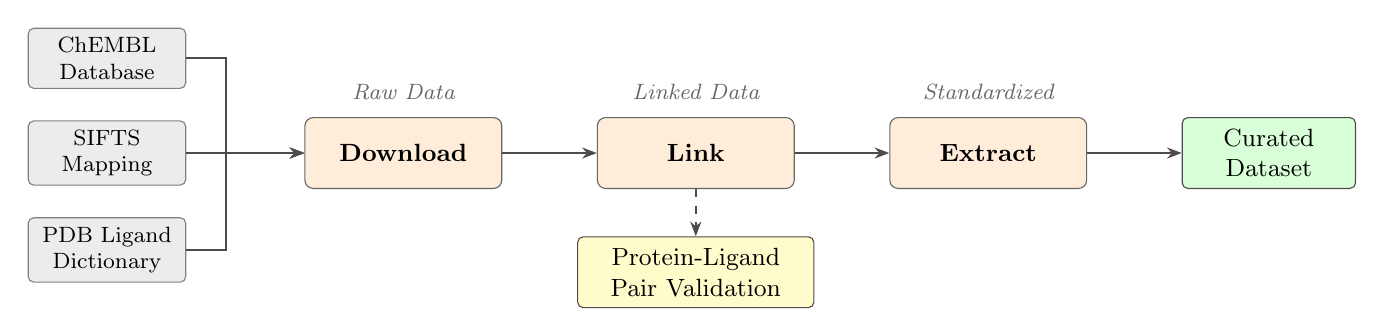
\begin{tikzpicture}[
    node distance=0.8cm and 1.2cm,
    box/.style={rectangle, draw=black!70, fill=blue!8, minimum width=2.2cm, minimum height=0.9cm, align=center, rounded corners=2pt, font=\small},
    databox/.style={rectangle, draw=black!50, fill=gray!15, minimum width=2cm, minimum height=0.7cm, align=center, rounded corners=2pt, font=\footnotesize},
    phase/.style={rectangle, draw=black!60, fill=orange!15, minimum width=2.5cm, minimum height=0.9cm, align=center, rounded corners=3pt, font=\small\bfseries},
    arrow/.style={-{Stealth[scale=0.8]}, thick, black!70},
    label/.style={font=\footnotesize\itshape, text=black!60}
]

% Data sources (left)
\node[databox] (chembl) {ChEMBL\\Database};
\node[databox, below=0.4cm of chembl] (sifts) {SIFTS\\Mapping};
\node[databox, below=0.4cm of sifts] (pdb) {PDB Ligand\\Dictionary};

% Phases
\node[phase, right=1.5cm of sifts] (download) {Download};
\node[phase, right=1.2cm of download] (link) {Link};
\node[phase, right=1.2cm of link] (extract) {Extract};

% Output
\node[box, right=1.2cm of extract, fill=green!15] (output) {Curated\\Dataset};

% Validation box
\node[box, below=0.6cm of link, fill=yellow!20, minimum width=3cm] (validate) {Protein-Ligand\\Pair Validation};

% Arrows from sources to download
\draw[arrow] (chembl.east) -- ++(0.5,0) |- (download.west);
\draw[arrow] (sifts.east) -- (download.west);
\draw[arrow] (pdb.east) -- ++(0.5,0) |- (download.west);

% Arrows between phases
\draw[arrow] (download) -- (link);
\draw[arrow] (link) -- (extract);
\draw[arrow] (extract) -- (output);

% Validation arrow
\draw[arrow, dashed] (link.south) -- (validate.north);

% Labels
\node[label, above=0.1cm of download] {Raw Data};
\node[label, above=0.1cm of link] {Linked Data};
\node[label, above=0.1cm of extract] {Standardized};

\end{tikzpicture}
\caption{\textbf{ChEMBL-PDB Linker pipeline architecture.} The pipeline integrates ChEMBL bioactivity data, SIFTS UniProt-PDB mappings, and PDB ligand information through three phases. The critical protein-ligand pair validation step (dashed box) ensures that matched protein-ligand pairs co-occur in the same crystal structure.}
\label{fig:pipeline}
\end{figure}

\subsection{Quality Filters}

The pipeline applies configurable quality filters:
\begin{itemize}
    \item \textbf{ChEMBL confidence score $\geq$ 9}: Ensures single-protein targets with high-confidence target assignments.
    \item \textbf{Activity types}: IC$_{50}$, K$_i$, K$_d$, and EC$_{50}$ measurements.
    \item \textbf{PDB resolution $\leq$ 3.5 \angstrom}: Ensures structural quality of protein-ligand complexes.
    \item \textbf{InChIKey matching}: Full 27-character matching (configurable to 14-character connectivity layer for stereoisomer coverage).
\end{itemize}

% ============================================================================
% RESULTS
% ============================================================================
\section{Results}

\subsection{Dataset Statistics}

The ChEMBL-PDB Linker dataset contains 98,500 validated protein-ligand pairs with associated bioactivity measurements (Table~\ref{tab:statistics}). The dataset spans 8,946 unique compounds, 1,297 target proteins, and 14,700 PDB structures.

\begin{table}[h]
\centering
\caption{\textbf{ChEMBL-PDB Linker dataset statistics.}}
\label{tab:statistics}
\begin{tabular}{@{}lr@{}}
\toprule
\textbf{Metric} & \textbf{Value} \\
\midrule
Validated protein-ligand pairs & 98,500 \\
Unique compounds & 8,946 \\
Unique target proteins & 1,297 \\
Unique PDB structures & 14,700 \\
Activity types & IC$_{50}$, K$_i$, K$_d$, EC$_{50}$ \\
Resolution range & 0.8--3.5 \angstrom \\
\bottomrule
\end{tabular}
\end{table}

\subsection{Validation Effectiveness}

The protein-ligand pair validation step is critical for dataset quality. Without validation, naive InChIKey matching produces matches where a ligand appears in a PDB structure that does not contain the target protein. Our validation eliminates approximately 99\% of these false positives, retaining only pairs where the PDB structure contains both entities.

\subsection{Comparison with PDBbind}

Table~\ref{tab:comparison} compares ChEMBL-PDB Linker with PDBbind. Our dataset is approximately five times larger while offering full automation, reproducibility, and on-demand regeneration capabilities.

\begin{table}[h]
\centering
\caption{\textbf{Comparison with PDBbind.}}
\label{tab:comparison}
\begin{tabular}{@{}lll@{}}
\toprule
\textbf{Feature} & \textbf{ChEMBL-PDB Linker} & \textbf{PDBbind} \\
\midrule
Dataset size & $\sim$98,500 pairs & $\sim$20,000 complexes \\
Bioactivity source & ChEMBL database & Literature curation \\
Structure source & PDB & PDB \\
Update frequency & On-demand & Annual \\
Reproducibility & Fully automated & Manual curation \\
Validation method & Algorithmic pair verification & Expert review \\
License & MIT (open source) & Academic license \\
\bottomrule
\end{tabular}
\end{table}

% ============================================================================
% AVAILABILITY
% ============================================================================
\section{Availability and Implementation}

ChEMBL-PDB Linker is implemented in Python and available as an open-source package:

\begin{itemize}
    \item \textbf{Repository}: \url{https://github.com/HFooladi/chembl-pdb-linker}
    \item \textbf{License}: MIT
    \item \textbf{Installation}: \texttt{pip install chembl-pdb-linker}
    \item \textbf{Usage}: \texttt{chembl-pdb-linker run} (complete pipeline)
\end{itemize}

The pipeline is configurable via YAML files, allowing users to adjust confidence thresholds, activity types, resolution cutoffs, and matching strategies. Output is provided in Parquet format for efficient storage and analysis.

% ============================================================================
% CONCLUSION
% ============================================================================
\section{Conclusion}

ChEMBL-PDB Linker provides a scalable, reproducible solution for linking bioactivity data with validated protein-ligand structures. The protein-ligand pair validation methodology ensures data quality while the automated pipeline enables on-demand dataset generation with the latest ChEMBL and PDB releases.

The dataset is suitable for training machine learning models for binding affinity prediction, virtual screening benchmarks, and structure-activity relationship studies. Future extensions may include integration with additional bioactivity databases, fragment-based screening sets, and covalent ligand complexes.

% ============================================================================
% ACKNOWLEDGMENTS
% ============================================================================
\section*{Acknowledgments}

The author thanks the ChEMBL, PDB, and SIFTS teams for maintaining these invaluable public resources.

% ============================================================================
% DATA AVAILABILITY
% ============================================================================
\section*{Data Availability}

The ChEMBL-PDB Linker software and generated datasets are freely available at \url{https://github.com/HFooladi/chembl-pdb-linker} under the MIT license.

% ============================================================================
% REFERENCES
% ============================================================================
\bibliographystyle{unsrtnat}
\bibliography{references}

\end{document}
